\documentclass[]{article}
\usepackage{amsmath}
\usepackage{amsthm}
\usepackage{listings}
\usepackage{graphicx} %for the fugures
\usepackage{cleveref} %for the cref command

\title{Practical Lab Numerical Computing Computational Finance \\Bachelor-Worksheet 2}
\author{Lukas Troska, Ilja Kalmykov}
\date{}
\setlength{\parindent}{0pt}

\begin{document}

\maketitle \section*{Task 1} Simulating the price of a call-option leads to
increasing mean value with larger $\sigma$ of the normal distribution. This is
due to the price of the call-option
\begin{eqnarray*}
V_{call}\left(S,T\right) & = &\max \lbrace S(T)-K,0 \rbrace
\end{eqnarray*}

always being positive. See task1.cpp,
task1.plot and \cref{fig:Task1} for details.
\begin{figure}[!ht]
% GNUPLOT: LaTeX picture with Postscript
\begingroup
  \makeatletter
  \providecommand\color[2][]{%
    \GenericError{(gnuplot) \space\space\space\@spaces}{%
      Package color not loaded in conjunction with
      terminal option `colourtext'%
    }{See the gnuplot documentation for explanation.%
    }{Either use 'blacktext' in gnuplot or load the package
      color.sty in LaTeX.}%
    \renewcommand\color[2][]{}%
  }%
  \providecommand\includegraphics[2][]{%
    \GenericError{(gnuplot) \space\space\space\@spaces}{%
      Package graphicx or graphics not loaded%
    }{See the gnuplot documentation for explanation.%
    }{The gnuplot epslatex terminal needs graphicx.sty or graphics.sty.}%
    \renewcommand\includegraphics[2][]{}%
  }%
  \providecommand\rotatebox[2]{#2}%
  \@ifundefined{ifGPcolor}{%
    \newif\ifGPcolor
    \GPcolortrue
  }{}%
  \@ifundefined{ifGPblacktext}{%
    \newif\ifGPblacktext
    \GPblacktexttrue
  }{}%
  % define a \g@addto@macro without @ in the name:
  \let\gplgaddtomacro\g@addto@macro
  % define empty templates for all commands taking text:
  \gdef\gplbacktext{}%
  \gdef\gplfronttext{}%
  \makeatother
  \ifGPblacktext
    % no textcolor at all
    \def\colorrgb#1{}%
    \def\colorgray#1{}%
  \else
    % gray or color?
    \ifGPcolor
      \def\colorrgb#1{\color[rgb]{#1}}%
      \def\colorgray#1{\color[gray]{#1}}%
      \expandafter\def\csname LTw\endcsname{\color{white}}%
      \expandafter\def\csname LTb\endcsname{\color{black}}%
      \expandafter\def\csname LTa\endcsname{\color{black}}%
      \expandafter\def\csname LT0\endcsname{\color[rgb]{1,0,0}}%
      \expandafter\def\csname LT1\endcsname{\color[rgb]{0,1,0}}%
      \expandafter\def\csname LT2\endcsname{\color[rgb]{0,0,1}}%
      \expandafter\def\csname LT3\endcsname{\color[rgb]{1,0,1}}%
      \expandafter\def\csname LT4\endcsname{\color[rgb]{0,1,1}}%
      \expandafter\def\csname LT5\endcsname{\color[rgb]{1,1,0}}%
      \expandafter\def\csname LT6\endcsname{\color[rgb]{0,0,0}}%
      \expandafter\def\csname LT7\endcsname{\color[rgb]{1,0.3,0}}%
      \expandafter\def\csname LT8\endcsname{\color[rgb]{0.5,0.5,0.5}}%
    \else
      % gray
      \def\colorrgb#1{\color{black}}%
      \def\colorgray#1{\color[gray]{#1}}%
      \expandafter\def\csname LTw\endcsname{\color{white}}%
      \expandafter\def\csname LTb\endcsname{\color{black}}%
      \expandafter\def\csname LTa\endcsname{\color{black}}%
      \expandafter\def\csname LT0\endcsname{\color{black}}%
      \expandafter\def\csname LT1\endcsname{\color{black}}%
      \expandafter\def\csname LT2\endcsname{\color{black}}%
      \expandafter\def\csname LT3\endcsname{\color{black}}%
      \expandafter\def\csname LT4\endcsname{\color{black}}%
      \expandafter\def\csname LT5\endcsname{\color{black}}%
      \expandafter\def\csname LT6\endcsname{\color{black}}%
      \expandafter\def\csname LT7\endcsname{\color{black}}%
      \expandafter\def\csname LT8\endcsname{\color{black}}%
    \fi
  \fi
  \setlength{\unitlength}{0.0500bp}%
  \begin{picture}(7200.00,5040.00)%
    \gplgaddtomacro\gplbacktext{%
      \csname LTb\endcsname%
      \put(814,704){\makebox(0,0)[r]{\strut{} 0}}%
      \csname LTb\endcsname%
      \put(814,1382){\makebox(0,0)[r]{\strut{} 5}}%
      \csname LTb\endcsname%
      \put(814,2061){\makebox(0,0)[r]{\strut{} 10}}%
      \csname LTb\endcsname%
      \put(814,2739){\makebox(0,0)[r]{\strut{} 15}}%
      \csname LTb\endcsname%
      \put(814,3418){\makebox(0,0)[r]{\strut{} 20}}%
      \csname LTb\endcsname%
      \put(814,4096){\makebox(0,0)[r]{\strut{} 25}}%
      \csname LTb\endcsname%
      \put(814,4775){\makebox(0,0)[r]{\strut{} 30}}%
      \csname LTb\endcsname%
      \put(1532,484){\makebox(0,0){\strut{} 0}}%
      \csname LTb\endcsname%
      \put(2703,484){\makebox(0,0){\strut{} 0.2}}%
      \csname LTb\endcsname%
      \put(3875,484){\makebox(0,0){\strut{} 0.4}}%
      \csname LTb\endcsname%
      \put(5046,484){\makebox(0,0){\strut{} 0.6}}%
      \csname LTb\endcsname%
      \put(6217,484){\makebox(0,0){\strut{} 0.8}}%
      \put(176,2739){\rotatebox{-270}{\makebox(0,0){\strut{}mean-estimate}}}%
      \put(3874,154){\makebox(0,0){\strut{}$\sigma$}}%
    }%
    \gplgaddtomacro\gplfronttext{%
    }%
    \gplbacktext
    \put(0,0){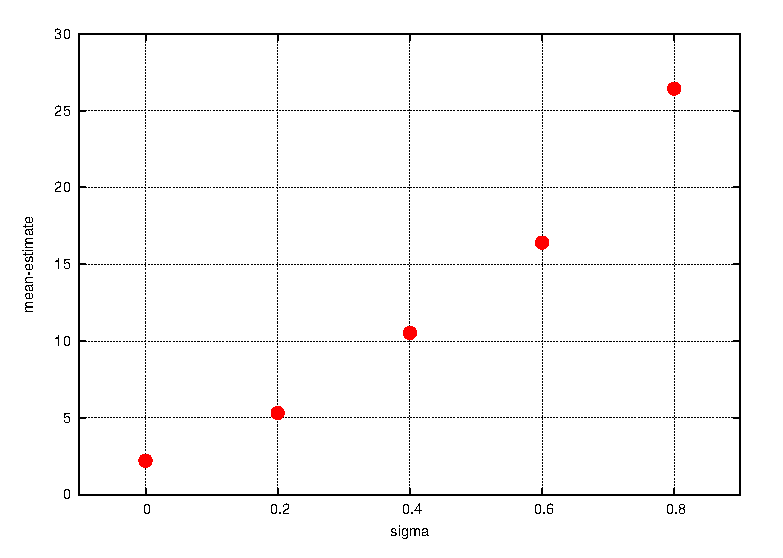
\includegraphics{task1Plot}}%
    \gplfronttext
  \end{picture}%
\endgroup

\caption{Mean-Estimate for the call-option prices for different values of
$\sigma$.}
\label{fig:Task1}
\end{figure}


\section*{Task 2} See task2.cpp for code. As we can see in the sample output
\cref{lst:Task2} below, the variance does not depend on $\Delta t$, since the
small differences can be caused by the (relatively) small sample size of N=1000
of the geometric brownian motions.
\begin{lstlisting}[caption = estimated $\mu$ and $\sigma$ for
different values of $\Delta t$ and N = 1.0E3, captionpos=b, label=lst:Task2] 
delta t = 2.000e-001 mean = 2.874e+000 variance = 3.811e+000
delta t = 4.000e-001 mean = 2.727e+000 variance = 3.429e+000
delta t = 5.000e-001 mean = 3.001e+000 variance = 3.752e+000
delta t = 1.000e+000 mean = 2.847e+000 variance = 3.747e+000
delta t = 2.000e+000 mean = 3.214e+000 variance = 3.885e+000
\end{lstlisting}

\section*{Task 3}
\begin{eqnarray*}
\cfrac{1}{\sqrt{2\pi}}\int_{\chi}^{\infty}K\exp\left(-\cfrac{s^2}{2}\right)ds &
= & \cfrac{1}{\sqrt{2\pi}}\left(\int_{-\infty}^{\infty}K\exp\left(-\cfrac{s^2}{2}\right)ds
- \int_{\infty}^{\chi}K\exp\left(-\cfrac{s^2}{2}\right)ds \right) \\
& = & K\left(1 - \Phi(\chi)\right) = K \Phi(-\chi)
\end{eqnarray*}

\section*{Task 4}
See task4.cpp, task4.plot and \cref{fig:Task4} for details. 

\begin{figure}[!ht]
% GNUPLOT: LaTeX picture with Postscript
\begingroup
  \makeatletter
  \providecommand\color[2][]{%
    \GenericError{(gnuplot) \space\space\space\@spaces}{%
      Package color not loaded in conjunction with
      terminal option `colourtext'%
    }{See the gnuplot documentation for explanation.%
    }{Either use 'blacktext' in gnuplot or load the package
      color.sty in LaTeX.}%
    \renewcommand\color[2][]{}%
  }%
  \providecommand\includegraphics[2][]{%
    \GenericError{(gnuplot) \space\space\space\@spaces}{%
      Package graphicx or graphics not loaded%
    }{See the gnuplot documentation for explanation.%
    }{The gnuplot epslatex terminal needs graphicx.sty or graphics.sty.}%
    \renewcommand\includegraphics[2][]{}%
  }%
  \providecommand\rotatebox[2]{#2}%
  \@ifundefined{ifGPcolor}{%
    \newif\ifGPcolor
    \GPcolortrue
  }{}%
  \@ifundefined{ifGPblacktext}{%
    \newif\ifGPblacktext
    \GPblacktexttrue
  }{}%
  % define a \g@addto@macro without @ in the name:
  \let\gplgaddtomacro\g@addto@macro
  % define empty templates for all commands taking text:
  \gdef\gplbacktext{}%
  \gdef\gplfronttext{}%
  \makeatother
  \ifGPblacktext
    % no textcolor at all
    \def\colorrgb#1{}%
    \def\colorgray#1{}%
  \else
    % gray or color?
    \ifGPcolor
      \def\colorrgb#1{\color[rgb]{#1}}%
      \def\colorgray#1{\color[gray]{#1}}%
      \expandafter\def\csname LTw\endcsname{\color{white}}%
      \expandafter\def\csname LTb\endcsname{\color{black}}%
      \expandafter\def\csname LTa\endcsname{\color{black}}%
      \expandafter\def\csname LT0\endcsname{\color[rgb]{1,0,0}}%
      \expandafter\def\csname LT1\endcsname{\color[rgb]{0,1,0}}%
      \expandafter\def\csname LT2\endcsname{\color[rgb]{0,0,1}}%
      \expandafter\def\csname LT3\endcsname{\color[rgb]{1,0,1}}%
      \expandafter\def\csname LT4\endcsname{\color[rgb]{0,1,1}}%
      \expandafter\def\csname LT5\endcsname{\color[rgb]{1,1,0}}%
      \expandafter\def\csname LT6\endcsname{\color[rgb]{0,0,0}}%
      \expandafter\def\csname LT7\endcsname{\color[rgb]{1,0.3,0}}%
      \expandafter\def\csname LT8\endcsname{\color[rgb]{0.5,0.5,0.5}}%
    \else
      % gray
      \def\colorrgb#1{\color{black}}%
      \def\colorgray#1{\color[gray]{#1}}%
      \expandafter\def\csname LTw\endcsname{\color{white}}%
      \expandafter\def\csname LTb\endcsname{\color{black}}%
      \expandafter\def\csname LTa\endcsname{\color{black}}%
      \expandafter\def\csname LT0\endcsname{\color{black}}%
      \expandafter\def\csname LT1\endcsname{\color{black}}%
      \expandafter\def\csname LT2\endcsname{\color{black}}%
      \expandafter\def\csname LT3\endcsname{\color{black}}%
      \expandafter\def\csname LT4\endcsname{\color{black}}%
      \expandafter\def\csname LT5\endcsname{\color{black}}%
      \expandafter\def\csname LT6\endcsname{\color{black}}%
      \expandafter\def\csname LT7\endcsname{\color{black}}%
      \expandafter\def\csname LT8\endcsname{\color{black}}%
    \fi
  \fi
  \setlength{\unitlength}{0.0500bp}%
  \begin{picture}(7200.00,5040.00)%
    \gplgaddtomacro\gplbacktext{%
      \csname LTb\endcsname%
      \put(946,704){\makebox(0,0)[r]{\strut{} 0.1}}%
      \csname LTb\endcsname%
      \put(946,2740){\makebox(0,0)[r]{\strut{} 1}}%
      \csname LTb\endcsname%
      \put(946,4775){\makebox(0,0)[r]{\strut{} 10}}%
      \csname LTb\endcsname%
      \put(1078,484){\makebox(0,0){\strut{} 1}}%
      \csname LTb\endcsname%
      \put(2032,484){\makebox(0,0){\strut{} 10}}%
      \csname LTb\endcsname%
      \put(2986,484){\makebox(0,0){\strut{} 100}}%
      \csname LTb\endcsname%
      \put(3940,484){\makebox(0,0){\strut{} 1000}}%
      \csname LTb\endcsname%
      \put(4895,484){\makebox(0,0){\strut{} 10000}}%
      \csname LTb\endcsname%
      \put(5849,484){\makebox(0,0){\strut{} 100000}}%
      \csname LTb\endcsname%
      \put(6803,484){\makebox(0,0){\strut{} 1e+006}}%
      \put(176,2739){\rotatebox{-270}{\makebox(0,0){\strut{}$m_n$}}}%
      \put(3940,154){\makebox(0,0){\strut{}N}}%
    }%
    \gplgaddtomacro\gplfronttext{%
      \csname LTb\endcsname%
      \put(5816,4602){\makebox(0,0)[r]{\strut{}run 1}}%
      \csname LTb\endcsname%
      \put(5816,4382){\makebox(0,0)[r]{\strut{}run 2}}%
      \csname LTb\endcsname%
      \put(5816,4162){\makebox(0,0)[r]{\strut{}run 3}}%
      \csname LTb\endcsname%
      \put(5816,3942){\makebox(0,0)[r]{\strut{}run 4}}%
      \csname LTb\endcsname%
      \put(5816,3722){\makebox(0,0)[r]{\strut{}run 5}}%
    }%
    \gplbacktext
    \put(0,0){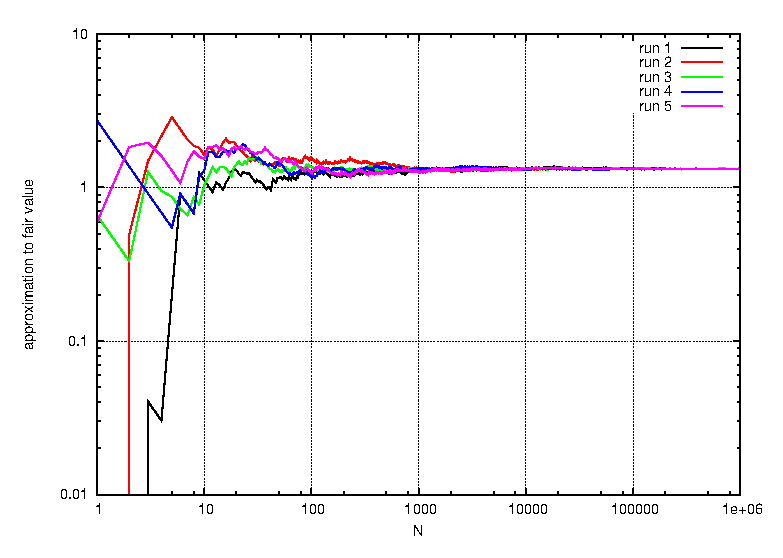
\includegraphics{task4Plot}}%
    \gplfronttext
  \end{picture}%
\endgroup

\caption{Approximation of $E\left[V_{call}(S_T,0)\right]$.}
\label{fig:Task4}
\end{figure}

\section*{Task 5} This formula is just a transformation. We have
\[\Phi(x)=\dfrac{1}{\sqrt{2\pi}}\int_{-\infty}^x
\exp\left({-\dfrac{t^2}{2}}\right)dt\] 
and thus
\[\Phi'(x)=\dfrac{1}{\sqrt{2\pi}}\exp\left({-\dfrac{x^2}{2}}\right)\]

For the derivative of the inverse we have in general, with $y = f(x)$:
\[\left(f^{-1}\right)'(y) = \left(f'\left(f^{-1}(y)\right)\right)^{-1}\]

and thus for the cumulative distribution function we get:
\begin{eqnarray}
\left(\Phi^{-1}\right)'(y) & = &
\left(\Phi'(\Phi^{-1}(y)\right)^{-1} \nonumber\\
\Leftrightarrow \quad \Phi'(\Phi^{-1}(y) & = & \left(\Phi^{-1}(y)\right)^{-1}
\label{equ:deriv}
\end{eqnarray}

Applying the transformation $s = \Phi^{-1}(t)$ and eq. (\ref{equ:deriv}) to 
\[\dfrac{1}{\sqrt{2\pi}}\int_{-\infty}^{\infty}f(s)\exp\left({-\dfrac{s^2}{2}}\right)ds\]
and using integration by substitution gives us:
\begin{eqnarray*}
\dfrac{1}{\sqrt{2\pi}}\int_{-\infty}^{\infty}f(s)\exp\left({-\dfrac{s^2}{2}}\right)ds
& = &
\int_{-\infty}^{\infty}f(s)\underbrace{\dfrac{1}{\sqrt{(2\pi)}}\exp\left({-\dfrac{s^2}{2}}\right)}_{\Phi'(\Phi^{-1})(t)
= \frac{1}{\left(\Phi^{-1}\right)'(t)}}ds \\
& =
&\int_{\Phi^{-1}(-\infty)}^{\Phi^{-1}(\infty)}f(\Phi^{-1}(t))\left(\Phi^{-1}\right)'(t)\cfrac{1}{\left(\Phi^{-1}\right)'(t)}ds
\\
& = &
\int_{1}^{0}f(\Phi^{-1}(t))ds
\end{eqnarray*}

\section*{Task 6} See task6.cpp for code. There is a relationship: You get the
nodes on level $(l+1)$ by taking the nodes on level $l$ and putting a new node
equidistant between two old nodes and also putting a new node equidistantly
between $0$ and the first old node, or $1$ and the last old node respectively.
Nodes positions are:
\begin{eqnarray*}
x_i = \cfrac{1}{N_l+1} = \cfrac{1}{2^l}
\end{eqnarray*}

\section*{Task 7}
See task7.cpp for code. We used GSL for Gauss-Legendre quadrature. The nodes for
the gaussian quadrature of degree $n$ are the roots of a polynomial of degree n
belonging to a class of orthogonal polynomials.

\section*{Task 8} See task8.cpp for code. Yes, there is a relationship: on level
$l+1$, we have the nodes from level $l$, and inbetween each "old" node we add a
new node as follows: if on level $l$ we have nodes $x_i,x_{i+1}$ at
\[ \dfrac{1}{2}\left(1-\cos\left(\dfrac{\pi i}{N_l+1}\right)\right)\]
 and
\[\dfrac{1}{2}\left(1-\cos\left(\dfrac{\pi(i+1)}{N_l+1}\right)\right)\]
 respectively, then on level $l+1$ they are node $x_{2i}$ and $x_{2i+2}$ respectively, since
\[\dfrac{i}{N_l+1}=\dfrac{2i}{N_{l+1}+1}\]
 (for $i+1$ analogously). We basically add nodes  $x_{i+0.5}$ for $0\le i \le
 N_l$.

\section*{Task 9}
See task9.cpp,
task9.plot for implementation. The convergence plots can be found in
\cref{fig:Task9}.

\begin{figure}[!ht]
% GNUPLOT: LaTeX picture with Postscript
\begingroup
  \makeatletter
  \providecommand\color[2][]{%
    \GenericError{(gnuplot) \space\space\space\@spaces}{%
      Package color not loaded in conjunction with
      terminal option `colourtext'%
    }{See the gnuplot documentation for explanation.%
    }{Either use 'blacktext' in gnuplot or load the package
      color.sty in LaTeX.}%
    \renewcommand\color[2][]{}%
  }%
  \providecommand\includegraphics[2][]{%
    \GenericError{(gnuplot) \space\space\space\@spaces}{%
      Package graphicx or graphics not loaded%
    }{See the gnuplot documentation for explanation.%
    }{The gnuplot epslatex terminal needs graphicx.sty or graphics.sty.}%
    \renewcommand\includegraphics[2][]{}%
  }%
  \providecommand\rotatebox[2]{#2}%
  \@ifundefined{ifGPcolor}{%
    \newif\ifGPcolor
    \GPcolortrue
  }{}%
  \@ifundefined{ifGPblacktext}{%
    \newif\ifGPblacktext
    \GPblacktexttrue
  }{}%
  % define a \g@addto@macro without @ in the name:
  \let\gplgaddtomacro\g@addto@macro
  % define empty templates for all commands taking text:
  \gdef\gplbacktext{}%
  \gdef\gplfronttext{}%
  \makeatother
  \ifGPblacktext
    % no textcolor at all
    \def\colorrgb#1{}%
    \def\colorgray#1{}%
  \else
    % gray or color?
    \ifGPcolor
      \def\colorrgb#1{\color[rgb]{#1}}%
      \def\colorgray#1{\color[gray]{#1}}%
      \expandafter\def\csname LTw\endcsname{\color{white}}%
      \expandafter\def\csname LTb\endcsname{\color{black}}%
      \expandafter\def\csname LTa\endcsname{\color{black}}%
      \expandafter\def\csname LT0\endcsname{\color[rgb]{1,0,0}}%
      \expandafter\def\csname LT1\endcsname{\color[rgb]{0,1,0}}%
      \expandafter\def\csname LT2\endcsname{\color[rgb]{0,0,1}}%
      \expandafter\def\csname LT3\endcsname{\color[rgb]{1,0,1}}%
      \expandafter\def\csname LT4\endcsname{\color[rgb]{0,1,1}}%
      \expandafter\def\csname LT5\endcsname{\color[rgb]{1,1,0}}%
      \expandafter\def\csname LT6\endcsname{\color[rgb]{0,0,0}}%
      \expandafter\def\csname LT7\endcsname{\color[rgb]{1,0.3,0}}%
      \expandafter\def\csname LT8\endcsname{\color[rgb]{0.5,0.5,0.5}}%
    \else
      % gray
      \def\colorrgb#1{\color{black}}%
      \def\colorgray#1{\color[gray]{#1}}%
      \expandafter\def\csname LTw\endcsname{\color{white}}%
      \expandafter\def\csname LTb\endcsname{\color{black}}%
      \expandafter\def\csname LTa\endcsname{\color{black}}%
      \expandafter\def\csname LT0\endcsname{\color{black}}%
      \expandafter\def\csname LT1\endcsname{\color{black}}%
      \expandafter\def\csname LT2\endcsname{\color{black}}%
      \expandafter\def\csname LT3\endcsname{\color{black}}%
      \expandafter\def\csname LT4\endcsname{\color{black}}%
      \expandafter\def\csname LT5\endcsname{\color{black}}%
      \expandafter\def\csname LT6\endcsname{\color{black}}%
      \expandafter\def\csname LT7\endcsname{\color{black}}%
      \expandafter\def\csname LT8\endcsname{\color{black}}%
    \fi
  \fi
  \setlength{\unitlength}{0.0500bp}%
  \begin{picture}(7200.00,5040.00)%
    \gplgaddtomacro\gplbacktext{%
      \colorrgb{1.00,1.00,1.00}%
      \put(1342,704){\makebox(0,0)[r]{\strut{} 1e-016}}%
      \colorrgb{1.00,1.00,1.00}%
      \put(1342,1213){\makebox(0,0)[r]{\strut{} 1e-014}}%
      \colorrgb{1.00,1.00,1.00}%
      \put(1342,1722){\makebox(0,0)[r]{\strut{} 1e-012}}%
      \colorrgb{1.00,1.00,1.00}%
      \put(1342,2231){\makebox(0,0)[r]{\strut{} 1e-010}}%
      \colorrgb{1.00,1.00,1.00}%
      \put(1342,2740){\makebox(0,0)[r]{\strut{} 1e-008}}%
      \colorrgb{1.00,1.00,1.00}%
      \put(1342,3248){\makebox(0,0)[r]{\strut{} 1e-006}}%
      \colorrgb{1.00,1.00,1.00}%
      \put(1342,3757){\makebox(0,0)[r]{\strut{} 0.0001}}%
      \colorrgb{1.00,1.00,1.00}%
      \put(1342,4266){\makebox(0,0)[r]{\strut{} 0.01}}%
      \colorrgb{1.00,1.00,1.00}%
      \put(1342,4775){\makebox(0,0)[r]{\strut{} 1}}%
      \colorrgb{1.00,1.00,1.00}%
      \put(1474,484){\makebox(0,0){\strut{} 1}}%
      \colorrgb{1.00,1.00,1.00}%
      \put(2806,484){\makebox(0,0){\strut{} 10}}%
      \colorrgb{1.00,1.00,1.00}%
      \put(4139,484){\makebox(0,0){\strut{} 100}}%
      \colorrgb{1.00,1.00,1.00}%
      \put(5471,484){\makebox(0,0){\strut{} 1000}}%
      \colorrgb{1.00,1.00,1.00}%
      \put(6803,484){\makebox(0,0){\strut{} 10000}}%
      \csname LTb\endcsname%
      \put(176,2739){\rotatebox{-270}{\makebox(0,0){\strut{}relative error}}}%
      \put(4138,154){\makebox(0,0){\strut{}num. nodes}}%
    }%
    \gplgaddtomacro\gplfronttext{%
      \csname LTb\endcsname%
      \put(5816,4602){\makebox(0,0)[r]{\strut{}monte-carlo}}%
      \csname LTb\endcsname%
      \put(5816,4382){\makebox(0,0)[r]{\strut{}trapezoidal}}%
      \csname LTb\endcsname%
      \put(5816,4162){\makebox(0,0)[r]{\strut{}clenshaw-curtis}}%
      \csname LTb\endcsname%
      \put(5816,3942){\makebox(0,0)[r]{\strut{}gauss-legendre}}%
    }%
    \gplbacktext
    \put(0,0){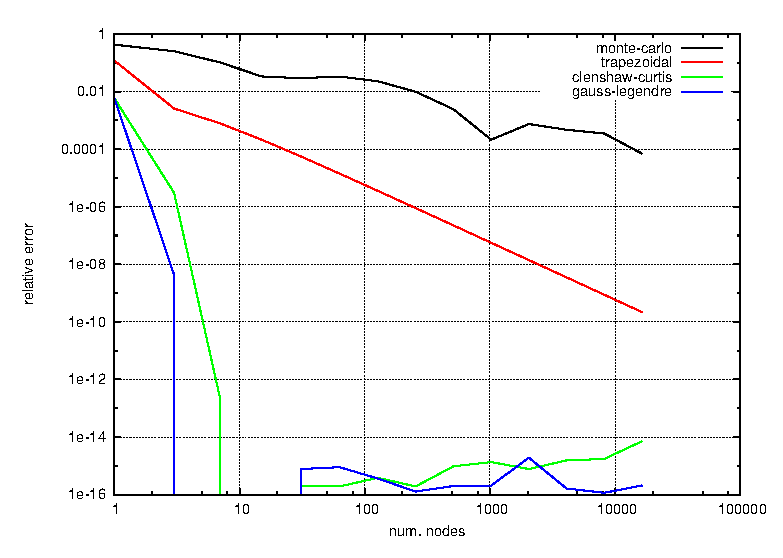
\includegraphics{task9Plot}}%
    \gplfronttext
  \end{picture}%
\endgroup

\caption{Relative error of different integration methods for
$1+\gamma\exp\left(\frac{1}{2}x\right)$ on $\left[0,1\right]$.}
\label{fig:Task9}
\end{figure}

\section*{Task 10} For the values
$S(0)=10,\mu=0.1,\sigma=0.2,T=2$ and $K=0$ we get an expected value of $\approx
12.21402758160169833921071994639$, for $K=10$ we get $\approx
2.6528094900348809449924483895885184345427710615192314$. See task10.cpp,
task10.plot for implementation. The convergence plots can be found in
\cref{fig:Task10_0} and \cref{fig:Task10_10}.

\begin{figure}[!ht]
% GNUPLOT: LaTeX picture with Postscript
\begingroup
  \makeatletter
  \providecommand\color[2][]{%
    \GenericError{(gnuplot) \space\space\space\@spaces}{%
      Package color not loaded in conjunction with
      terminal option `colourtext'%
    }{See the gnuplot documentation for explanation.%
    }{Either use 'blacktext' in gnuplot or load the package
      color.sty in LaTeX.}%
    \renewcommand\color[2][]{}%
  }%
  \providecommand\includegraphics[2][]{%
    \GenericError{(gnuplot) \space\space\space\@spaces}{%
      Package graphicx or graphics not loaded%
    }{See the gnuplot documentation for explanation.%
    }{The gnuplot epslatex terminal needs graphicx.sty or graphics.sty.}%
    \renewcommand\includegraphics[2][]{}%
  }%
  \providecommand\rotatebox[2]{#2}%
  \@ifundefined{ifGPcolor}{%
    \newif\ifGPcolor
    \GPcolortrue
  }{}%
  \@ifundefined{ifGPblacktext}{%
    \newif\ifGPblacktext
    \GPblacktexttrue
  }{}%
  % define a \g@addto@macro without @ in the name:
  \let\gplgaddtomacro\g@addto@macro
  % define empty templates for all commands taking text:
  \gdef\gplbacktext{}%
  \gdef\gplfronttext{}%
  \makeatother
  \ifGPblacktext
    % no textcolor at all
    \def\colorrgb#1{}%
    \def\colorgray#1{}%
  \else
    % gray or color?
    \ifGPcolor
      \def\colorrgb#1{\color[rgb]{#1}}%
      \def\colorgray#1{\color[gray]{#1}}%
      \expandafter\def\csname LTw\endcsname{\color{white}}%
      \expandafter\def\csname LTb\endcsname{\color{black}}%
      \expandafter\def\csname LTa\endcsname{\color{black}}%
      \expandafter\def\csname LT0\endcsname{\color[rgb]{1,0,0}}%
      \expandafter\def\csname LT1\endcsname{\color[rgb]{0,1,0}}%
      \expandafter\def\csname LT2\endcsname{\color[rgb]{0,0,1}}%
      \expandafter\def\csname LT3\endcsname{\color[rgb]{1,0,1}}%
      \expandafter\def\csname LT4\endcsname{\color[rgb]{0,1,1}}%
      \expandafter\def\csname LT5\endcsname{\color[rgb]{1,1,0}}%
      \expandafter\def\csname LT6\endcsname{\color[rgb]{0,0,0}}%
      \expandafter\def\csname LT7\endcsname{\color[rgb]{1,0.3,0}}%
      \expandafter\def\csname LT8\endcsname{\color[rgb]{0.5,0.5,0.5}}%
    \else
      % gray
      \def\colorrgb#1{\color{black}}%
      \def\colorgray#1{\color[gray]{#1}}%
      \expandafter\def\csname LTw\endcsname{\color{white}}%
      \expandafter\def\csname LTb\endcsname{\color{black}}%
      \expandafter\def\csname LTa\endcsname{\color{black}}%
      \expandafter\def\csname LT0\endcsname{\color{black}}%
      \expandafter\def\csname LT1\endcsname{\color{black}}%
      \expandafter\def\csname LT2\endcsname{\color{black}}%
      \expandafter\def\csname LT3\endcsname{\color{black}}%
      \expandafter\def\csname LT4\endcsname{\color{black}}%
      \expandafter\def\csname LT5\endcsname{\color{black}}%
      \expandafter\def\csname LT6\endcsname{\color{black}}%
      \expandafter\def\csname LT7\endcsname{\color{black}}%
      \expandafter\def\csname LT8\endcsname{\color{black}}%
    \fi
  \fi
  \setlength{\unitlength}{0.0500bp}%
  \begin{picture}(7200.00,5040.00)%
    \gplgaddtomacro\gplbacktext{%
      \colorrgb{1.00,1.00,1.00}%
      \put(1342,704){\makebox(0,0)[r]{\strut{} 1e-007}}%
      \colorrgb{1.00,1.00,1.00}%
      \put(1342,1213){\makebox(0,0)[r]{\strut{} 1e-006}}%
      \colorrgb{1.00,1.00,1.00}%
      \put(1342,1722){\makebox(0,0)[r]{\strut{} 1e-005}}%
      \colorrgb{1.00,1.00,1.00}%
      \put(1342,2231){\makebox(0,0)[r]{\strut{} 0.0001}}%
      \colorrgb{1.00,1.00,1.00}%
      \put(1342,2740){\makebox(0,0)[r]{\strut{} 0.001}}%
      \colorrgb{1.00,1.00,1.00}%
      \put(1342,3248){\makebox(0,0)[r]{\strut{} 0.01}}%
      \colorrgb{1.00,1.00,1.00}%
      \put(1342,3757){\makebox(0,0)[r]{\strut{} 0.1}}%
      \colorrgb{1.00,1.00,1.00}%
      \put(1342,4266){\makebox(0,0)[r]{\strut{} 1}}%
      \colorrgb{1.00,1.00,1.00}%
      \put(1342,4775){\makebox(0,0)[r]{\strut{} 10}}%
      \colorrgb{1.00,1.00,1.00}%
      \put(1474,484){\makebox(0,0){\strut{} 1}}%
      \colorrgb{1.00,1.00,1.00}%
      \put(2806,484){\makebox(0,0){\strut{} 10}}%
      \colorrgb{1.00,1.00,1.00}%
      \put(4139,484){\makebox(0,0){\strut{} 100}}%
      \colorrgb{1.00,1.00,1.00}%
      \put(5471,484){\makebox(0,0){\strut{} 1000}}%
      \colorrgb{1.00,1.00,1.00}%
      \put(6803,484){\makebox(0,0){\strut{} 10000}}%
      \csname LTb\endcsname%
      \put(176,2739){\rotatebox{-270}{\makebox(0,0){\strut{}relative error}}}%
      \put(4138,154){\makebox(0,0){\strut{}num nodes}}%
    }%
    \gplgaddtomacro\gplfronttext{%
      \csname LTb\endcsname%
      \put(5816,4602){\makebox(0,0)[r]{\strut{}monte-carlo}}%
      \csname LTb\endcsname%
      \put(5816,4382){\makebox(0,0)[r]{\strut{}trapezoidal}}%
      \csname LTb\endcsname%
      \put(5816,4162){\makebox(0,0)[r]{\strut{}clenshaw-curtis}}%
      \csname LTb\endcsname%
      \put(5816,3942){\makebox(0,0)[r]{\strut{}gauss-legendre}}%
    }%
    \gplbacktext
    \put(0,0){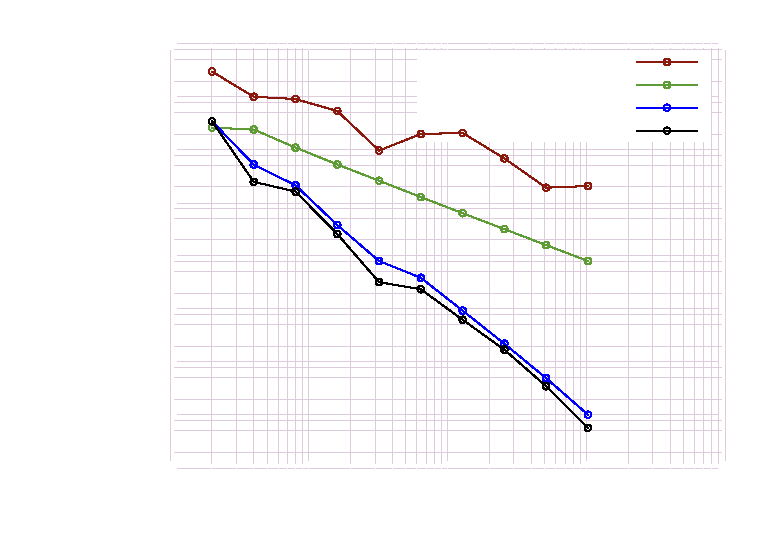
\includegraphics{task10_0Plot}}%
    \gplfronttext
  \end{picture}%
\endgroup

\caption{Relative error of different integration methods for
$f_{call}\circ \Phi^{-1}$ with $K = 0$.}
\label{fig:Task10_0}
\end{figure}

\begin{figure}[!ht]
% GNUPLOT: LaTeX picture with Postscript
\begingroup
  \makeatletter
  \providecommand\color[2][]{%
    \GenericError{(gnuplot) \space\space\space\@spaces}{%
      Package color not loaded in conjunction with
      terminal option `colourtext'%
    }{See the gnuplot documentation for explanation.%
    }{Either use 'blacktext' in gnuplot or load the package
      color.sty in LaTeX.}%
    \renewcommand\color[2][]{}%
  }%
  \providecommand\includegraphics[2][]{%
    \GenericError{(gnuplot) \space\space\space\@spaces}{%
      Package graphicx or graphics not loaded%
    }{See the gnuplot documentation for explanation.%
    }{The gnuplot epslatex terminal needs graphicx.sty or graphics.sty.}%
    \renewcommand\includegraphics[2][]{}%
  }%
  \providecommand\rotatebox[2]{#2}%
  \@ifundefined{ifGPcolor}{%
    \newif\ifGPcolor
    \GPcolortrue
  }{}%
  \@ifundefined{ifGPblacktext}{%
    \newif\ifGPblacktext
    \GPblacktexttrue
  }{}%
  % define a \g@addto@macro without @ in the name:
  \let\gplgaddtomacro\g@addto@macro
  % define empty templates for all commands taking text:
  \gdef\gplbacktext{}%
  \gdef\gplfronttext{}%
  \makeatother
  \ifGPblacktext
    % no textcolor at all
    \def\colorrgb#1{}%
    \def\colorgray#1{}%
  \else
    % gray or color?
    \ifGPcolor
      \def\colorrgb#1{\color[rgb]{#1}}%
      \def\colorgray#1{\color[gray]{#1}}%
      \expandafter\def\csname LTw\endcsname{\color{white}}%
      \expandafter\def\csname LTb\endcsname{\color{black}}%
      \expandafter\def\csname LTa\endcsname{\color{black}}%
      \expandafter\def\csname LT0\endcsname{\color[rgb]{1,0,0}}%
      \expandafter\def\csname LT1\endcsname{\color[rgb]{0,1,0}}%
      \expandafter\def\csname LT2\endcsname{\color[rgb]{0,0,1}}%
      \expandafter\def\csname LT3\endcsname{\color[rgb]{1,0,1}}%
      \expandafter\def\csname LT4\endcsname{\color[rgb]{0,1,1}}%
      \expandafter\def\csname LT5\endcsname{\color[rgb]{1,1,0}}%
      \expandafter\def\csname LT6\endcsname{\color[rgb]{0,0,0}}%
      \expandafter\def\csname LT7\endcsname{\color[rgb]{1,0.3,0}}%
      \expandafter\def\csname LT8\endcsname{\color[rgb]{0.5,0.5,0.5}}%
    \else
      % gray
      \def\colorrgb#1{\color{black}}%
      \def\colorgray#1{\color[gray]{#1}}%
      \expandafter\def\csname LTw\endcsname{\color{white}}%
      \expandafter\def\csname LTb\endcsname{\color{black}}%
      \expandafter\def\csname LTa\endcsname{\color{black}}%
      \expandafter\def\csname LT0\endcsname{\color{black}}%
      \expandafter\def\csname LT1\endcsname{\color{black}}%
      \expandafter\def\csname LT2\endcsname{\color{black}}%
      \expandafter\def\csname LT3\endcsname{\color{black}}%
      \expandafter\def\csname LT4\endcsname{\color{black}}%
      \expandafter\def\csname LT5\endcsname{\color{black}}%
      \expandafter\def\csname LT6\endcsname{\color{black}}%
      \expandafter\def\csname LT7\endcsname{\color{black}}%
      \expandafter\def\csname LT8\endcsname{\color{black}}%
    \fi
  \fi
  \setlength{\unitlength}{0.0500bp}%
  \begin{picture}(7200.00,5040.00)%
    \gplgaddtomacro\gplbacktext{%
      \colorrgb{1.00,1.00,1.00}%
      \put(1342,704){\makebox(0,0)[r]{\strut{} 1e-07}}%
      \colorrgb{1.00,1.00,1.00}%
      \put(1342,1213){\makebox(0,0)[r]{\strut{} 1e-06}}%
      \colorrgb{1.00,1.00,1.00}%
      \put(1342,1722){\makebox(0,0)[r]{\strut{} 1e-05}}%
      \colorrgb{1.00,1.00,1.00}%
      \put(1342,2231){\makebox(0,0)[r]{\strut{} 0.0001}}%
      \colorrgb{1.00,1.00,1.00}%
      \put(1342,2740){\makebox(0,0)[r]{\strut{} 0.001}}%
      \colorrgb{1.00,1.00,1.00}%
      \put(1342,3248){\makebox(0,0)[r]{\strut{} 0.01}}%
      \colorrgb{1.00,1.00,1.00}%
      \put(1342,3757){\makebox(0,0)[r]{\strut{} 0.1}}%
      \colorrgb{1.00,1.00,1.00}%
      \put(1342,4266){\makebox(0,0)[r]{\strut{} 1}}%
      \colorrgb{1.00,1.00,1.00}%
      \put(1342,4775){\makebox(0,0)[r]{\strut{} 10}}%
      \colorrgb{1.00,1.00,1.00}%
      \put(1474,484){\makebox(0,0){\strut{} 1}}%
      \colorrgb{1.00,1.00,1.00}%
      \put(6803,484){\makebox(0,0){\strut{} 10}}%
      \csname LTb\endcsname%
      \put(176,2739){\rotatebox{-270}{\makebox(0,0){\strut{}relative error}}}%
      \put(4138,154){\makebox(0,0){\strut{}num nodes}}%
    }%
    \gplgaddtomacro\gplfronttext{%
      \csname LTb\endcsname%
      \put(5816,4602){\makebox(0,0)[r]{\strut{}monte-carlo}}%
      \csname LTb\endcsname%
      \put(5816,4382){\makebox(0,0)[r]{\strut{}trapezoidal}}%
      \csname LTb\endcsname%
      \put(5816,4162){\makebox(0,0)[r]{\strut{}clenshaw-curtis}}%
      \csname LTb\endcsname%
      \put(5816,3942){\makebox(0,0)[r]{\strut{}gauss-legendre}}%
    }%
    \gplbacktext
    \put(0,0){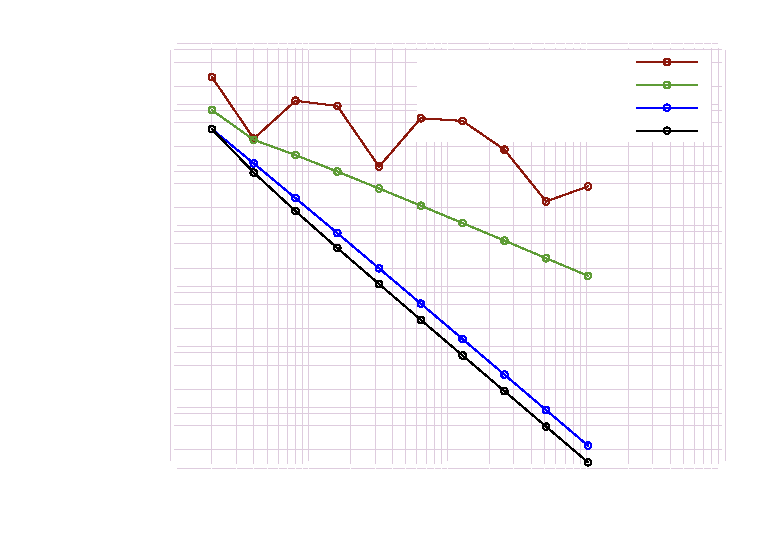
\includegraphics{task10_10Plot}}%
    \gplfronttext
  \end{picture}%
\endgroup

\caption{Relative error of different integration methods for
$f_{call}\circ \Phi^{-1}$ with $K = 10$.}
\label{fig:Task10_10}
\end{figure}

\end{document}
